\scanpage{117}
\begin{flushright}
Le 27 Mars 1968\\
17H 45\\
\end{flushright}

\begin{center}
\uline{Monsieur GROTHENDIECK}\\
\end{center}

\begin{enumerate}[label=\arabic*.]
\item Melle Zabardi me dit avoir refait dans le détail 6 pages de vos 17 pages de corrections. Elle pense avoir fini demain soir.

\item Mme Hakim ayant appris que les stencils sont stockés Rue de Lille a demandé à Melle Chardon 5 exemplaires de ``La vie Mathématiques en République Démocratique du Vietnam'' et propose de tirer des stencils électroniques.

\item Nous ferons déposer vendredi à Massy les stencils de votre manuscrit et de celui de Jussila.
\end{enumerate}

\figure{\makebox[\linewidth][r]{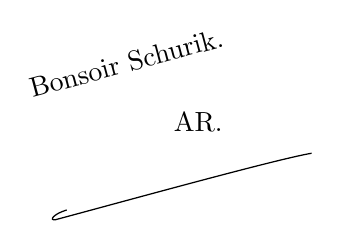
\begin{tikzpicture}[x=1em,y=1em]
\node[anchor=base west,inner sep=0,rotate=15] at (0,4.4) {\handwritten{\unsure{Bonsoir} Schurik.}};
\node[anchor=base west,inner sep=0] at (5.1,3.2) {\handwritten{\unsure{AR}.}};
\draw[line width=.45pt] (1.25,.35) .. controls (.75,.20) and (.60,-.05) .. (.85,0) .. controls (3.1,.60) and (8.8,2.18) .. (10.1,2.40);
\end{tikzpicture}}}
% archive sheet number: 116
